\documentclass{article}
\usepackage[utf8]{inputenc}
\usepackage{subfig}

%References
\usepackage{natbib}
%IMPORTANT use https://www.citationmachine.net/ if you need to generate references!
% \citep{reference} creates Harvard Style references throughout

%Colors
\usepackage{xcolor}

\usepackage[protrusion=true,expansion]{microtype}

%Code Markup
\usepackage[outputdir=cache]{minted}
%Syntax Highlighting Style
\definecolor{bggray}{RGB}{40,40,40}
%Macro to make a Syntax Highlighter For Java files 
%Use \javacode{filename.java} to insert a Java File W/ Syntax Highlighting file into the PDF
\newmintedfile[javacode]{java}{
	style=fruity,
	bgcolor=bggray,
	linenos,
	breaklines,
	tabsize=2,
	obeytabs
}

\newmintedfile[bashoutput]{txt}{
	style=fruity,
	bgcolor=lightgray,
	breaklines,
	tabsize=2,
	obeytabs
}

%Page Margins and stuff
\usepackage{geometry}
 \geometry{
 a4paper,
 total={170mm,257mm},
 left=20mm,
 }

%Pictures
\usepackage{graphicx}
\graphicspath{ {./images/} }

%Move the title position
\usepackage{titling}

\setlength{\droptitle}{-8.5em} %Up, near the top but not too high

\title{Assignment 2 -  CT3531 Networks \& Data Communications II}
\author{Daniel Hannon (19484286)}
\date{November 2021}

\begin{document}
	\maketitle
	\section{GNS3 Config}
		\begin{figure}[h!]
			\centering
			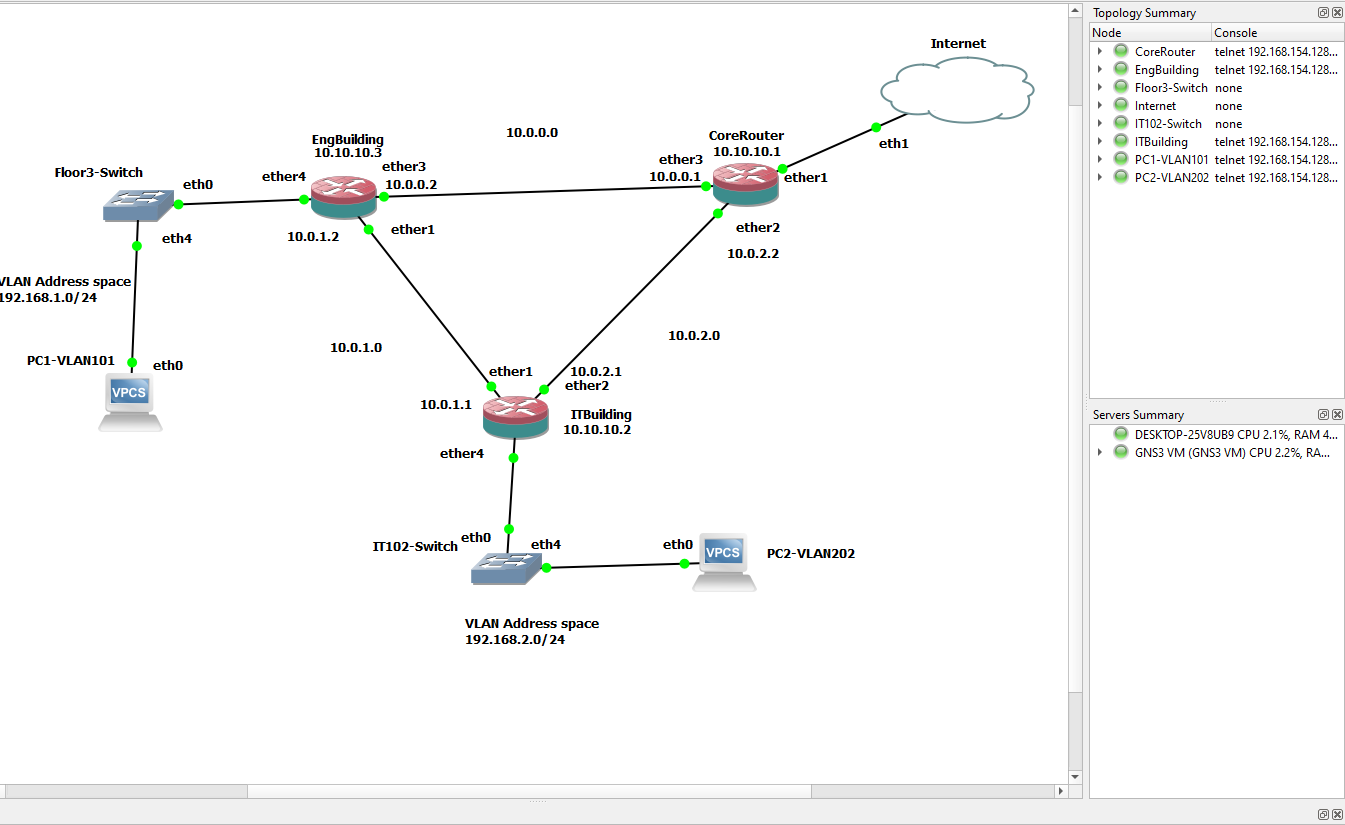
\includegraphics[width=0.8\textwidth]{gns3_config}
		\end{figure}
		\newpage
	\section{Router Configs}
		\begin{figure}[h!]
			\centering
			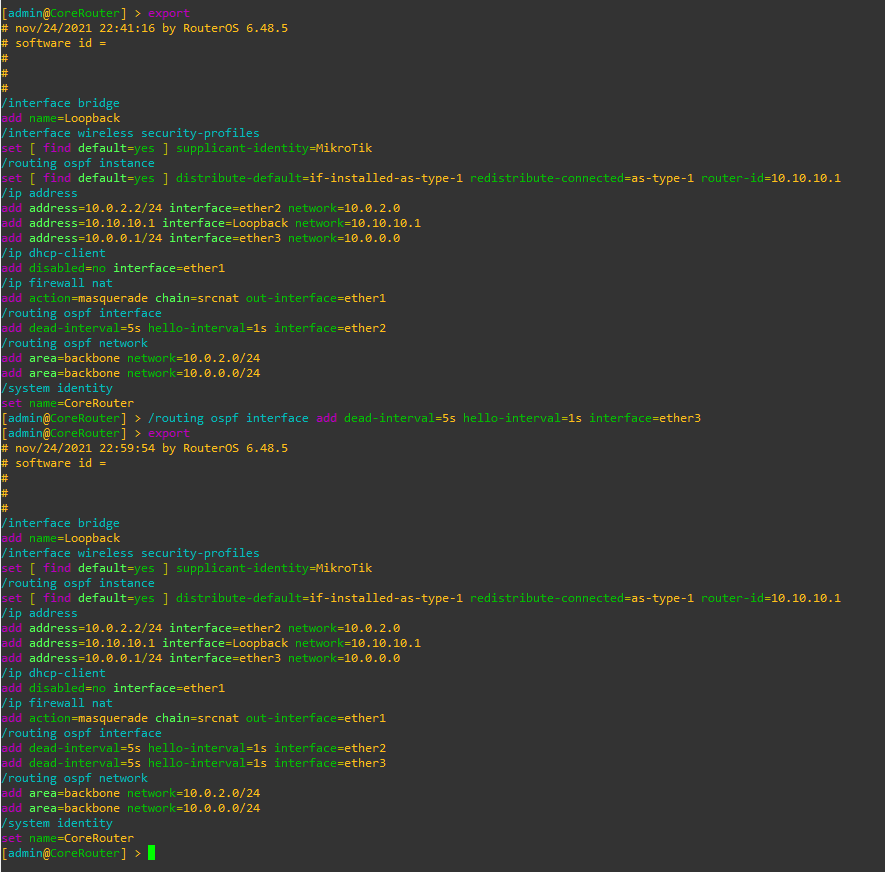
\includegraphics[width=0.7\textwidth]{core_router_config}
			\caption{Core Router Config}
		\end{figure}
		\begin{figure}[h!]
			\centering
			\begin{minipage}{0.5\textwidth}
				\centering
				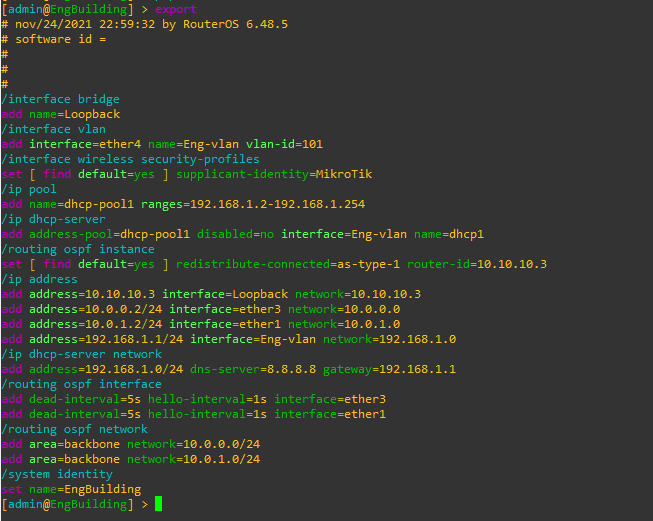
\includegraphics[width=0.9\textwidth]{eng_router_config}
				\caption{Engineering Router Config}
			\end{minipage}%
			\begin{minipage}{0.5\textwidth}
				\centering
				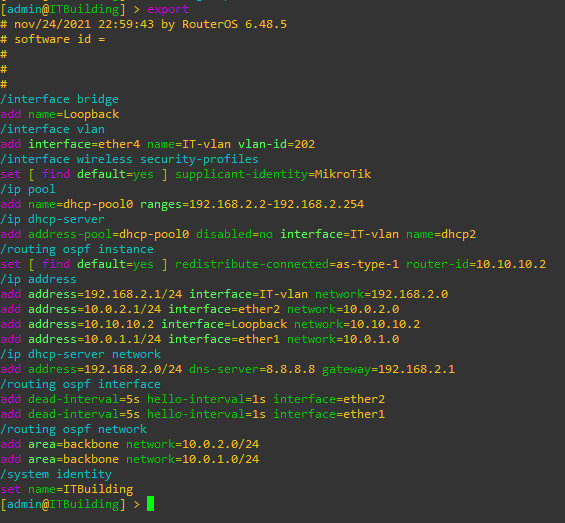
\includegraphics[width=0.9\textwidth]{it_router_config}
				\caption{IT Router Config}
			\end{minipage}
		\end{figure}
		\newpage
	\section{Loopback Ping Verification}
		\begin{figure}[h!]
			\centering
				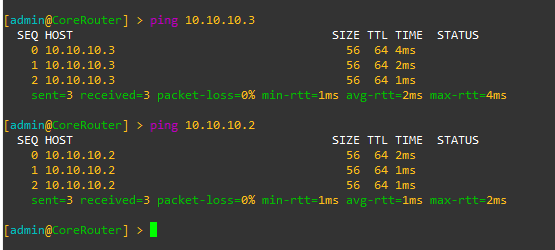
\includegraphics[width=0.9\textwidth]{core_loopback_pings}
				\caption{Core Loopback Pings}
		\end{figure}
		\begin{figure}[h!]
			\centering
				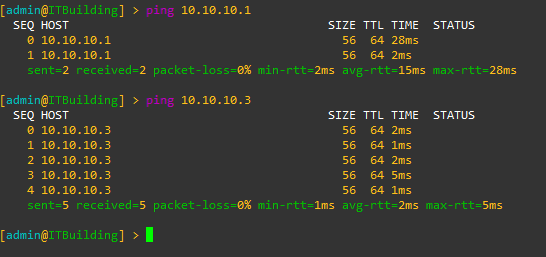
\includegraphics[width=0.9\textwidth]{it_loopback_pings}
				\caption{IT Loopback Pings}
		\end{figure}
		\begin{figure}[h!]
			\centering
				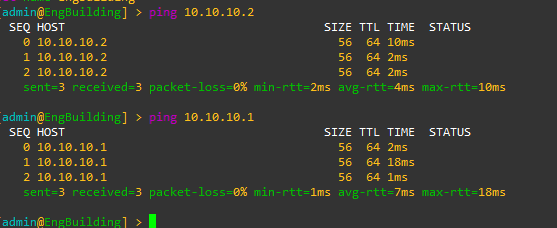
\includegraphics[width=0.9\textwidth]{eng_loopback_pings}
				\caption{Engineering Loopback Pings}
		\end{figure}
		\newpage
	\section{Routing Table Verification}
		\begin{figure}[h!]
			\begin{minipage}{0.5\textwidth}
				\centering
				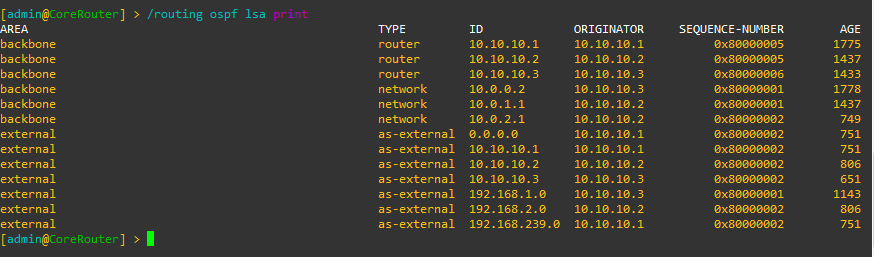
\includegraphics[width=0.9\textwidth]{core_routing_table}
			\end{minipage}%
			\begin{minipage}{0.5\textwidth}
				\centering
				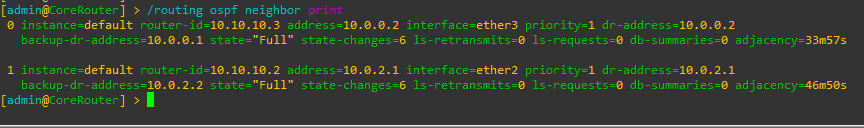
\includegraphics[width=0.9\textwidth]{core_neighbors}
			\end{minipage}
			\caption{Core Routing Table \& Neighbor list}
		\end{figure}
		\begin{figure}[h!]
			\begin{minipage}{0.5\textwidth}
				\centering
				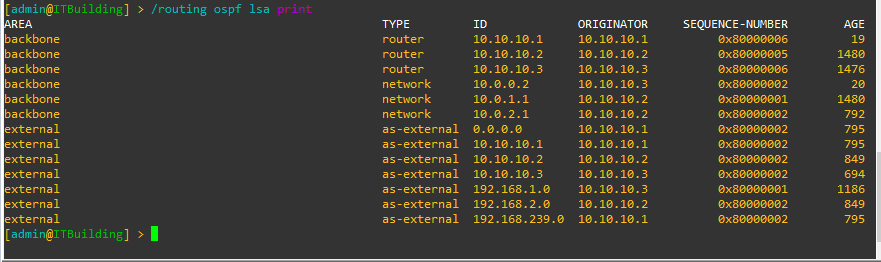
\includegraphics[width=0.9\textwidth]{it_routing_table}
			\end{minipage}%
			\begin{minipage}{0.5\textwidth}
				\centering
				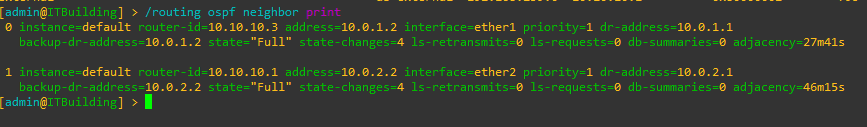
\includegraphics[width=0.9\textwidth]{it_neighbors}
			\end{minipage}
			\caption{IT Routing Table \& Neighbor list}
		\end{figure}
		\begin{figure}[h!]
			\begin{minipage}{0.5\textwidth}
				\centering
				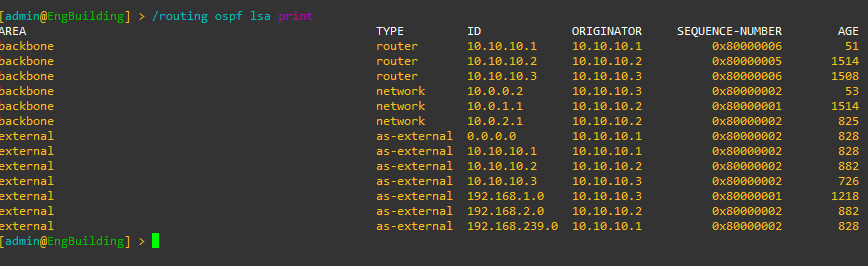
\includegraphics[width=0.9\textwidth]{eng_routing_table}
			\end{minipage}%
			\begin{minipage}{0.5\textwidth}
				\centering
				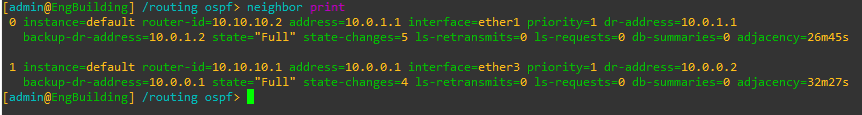
\includegraphics[width=0.9\textwidth]{eng_neighbors}
			\end{minipage}
			\caption{Engineering Routing Table \& Neighbor list}
		\end{figure}
	\section{Internet connection verification}
		\begin{figure}[h!]
			\centering
			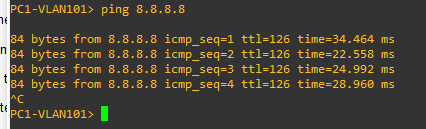
\includegraphics[width=0.8\textwidth]{pc1_internet_ping}
			\caption{PC1 Internet Ping}
		\end{figure}
		\begin{figure}[h!]
			\centering
			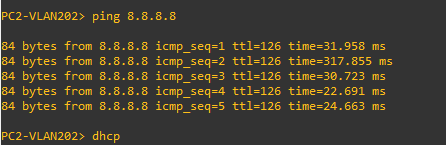
\includegraphics[width=0.8\textwidth]{pc2_internet_ping}
			\caption{PC2 Internet Ping}
		\end{figure}
		Proof the routers can reach the internet is trivial.
		\newpage
	\section{Step 12}
		If the routers were not configured correctly to perform OSPF neither the Engineering or IT routers would be able to connect to the internet as they would not know that there was a DHCP gateway on the core router. Furthermore, the computers on either the IT or Engineering network would be unable to communicate with eachother (or get a dynamically assigned ip address as they would be unable to reach the dns server (8.8.8.8) )\\
		The routers at IT and Engineering would no longer be able to communicate if the direct link was severed as they would not know of the other route.
	\section{Step 13}
		\begin{figure}[h!]
			\centering
			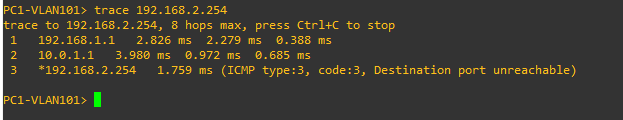
\includegraphics[width=0.8\textwidth]{step_13_trace}
		\end{figure}
		\begin{enumerate}
			\item 192.168.1.1 was the IP address of the Engineering Router
			\item 10.0.1.1 is the IP address of IT Router on the direct line between it and the engineering router
			\item 192.168.2.254 was the destination.
		\end{enumerate}
		\newpage
	\section{Step 15}
		\begin{figure}[h!]
			\centering
			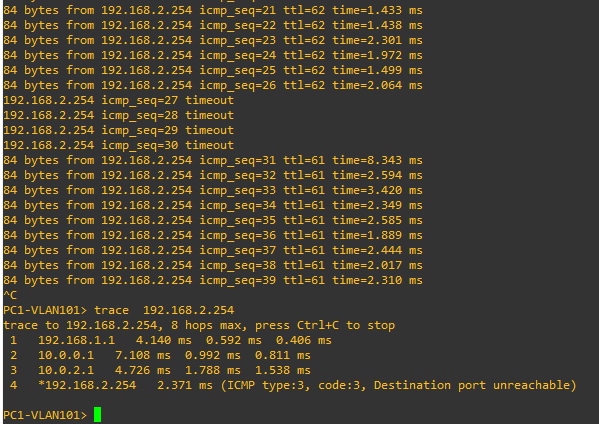
\includegraphics[width=0.8\textwidth]{step_15_trace_with_pings}
		\end{figure}
		Ultimately four pings failed, which spanned about six seconds in duration. which was expected considering the dead-interval and hello interval. The new route denotes:
		\begin{enumerate}
			\item The Engineering router
			\item Core Router
			\item IT Router
			\item The Destination PC
		\end{enumerate}
		\newpage
	\section{LSA\'s from reconnecting the routers directly again}
		\begin{figure}[h!]
			\centering
			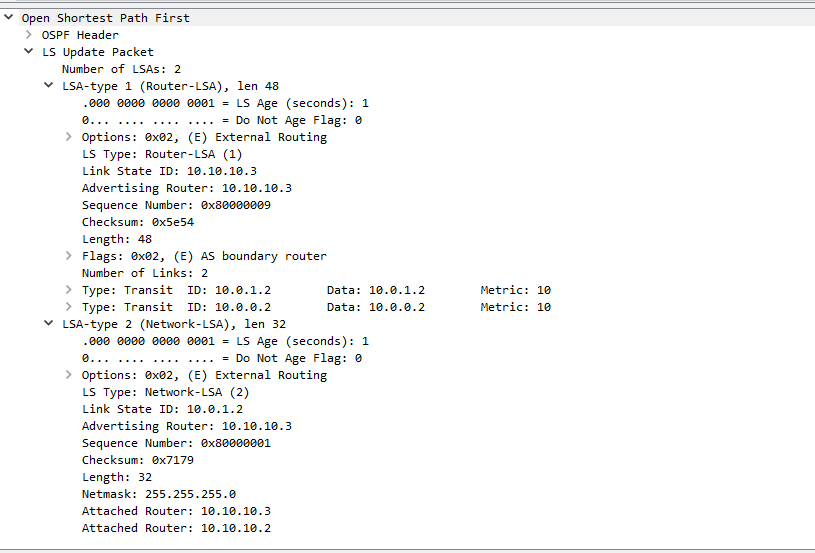
\includegraphics[width=0.8\textwidth]{first_lsa}
			\caption{First Link State Announcement}
		\end{figure}
		\begin{figure}[h!]
			\centering
			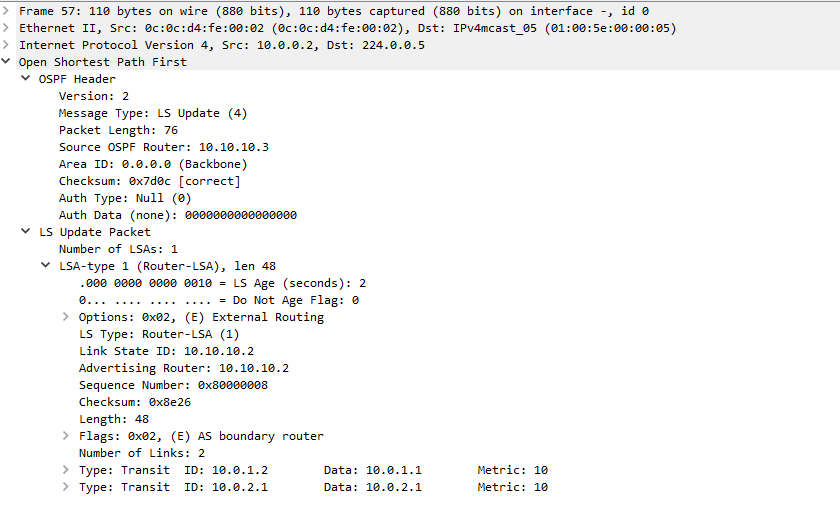
\includegraphics[width=0.8\textwidth]{second_lsa}
			\caption{Second Link State Announcement}
		\end{figure}
		\newpage
		\begin{figure}[h!]
			\centering
			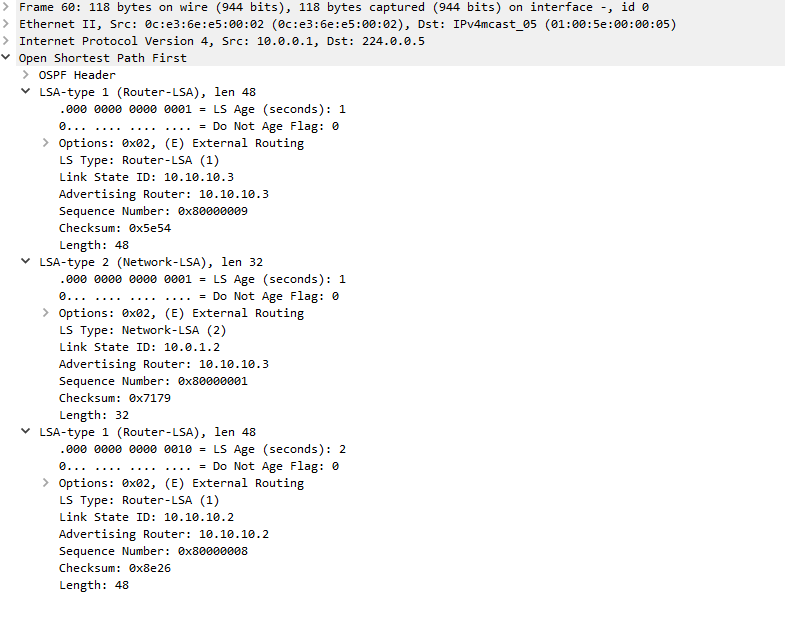
\includegraphics[width=0.8\textwidth]{lsa_ack}
			\caption{Link State Announcement ACK packet}
		\end{figure}
		The first LSA packet contained the list of routers the engineering router had a direct connection to. The second one contained the routes to them. and The final packet was an ACK from the core router to verify it recieved the data
	%Sets to Harvard Style and links the references file
	\bibliographystyle{agsm}
	\bibliography{references}
\end{document}